\begin{figure}[H]
  \centerline{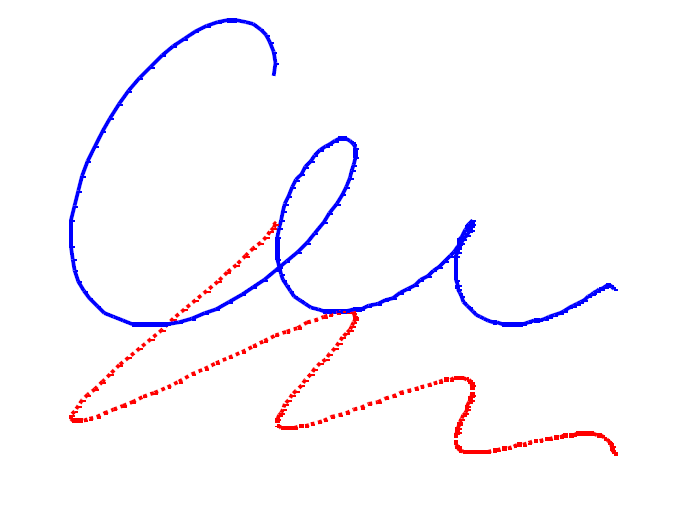
\includegraphics[width=0.8\textwidth]{Syslogo.PNG}}
\end{figure}

\noindent \bigskip

\centerline  {\fontfamily{phv}\fontsize{40}{50}\selectfont Systemtheorie Teil A} 

\noindent \medskip

\centerline  {\fontfamily{phv}\fontsize{20}{20}\selectfont  - Zeitkontinuierliche Signale und Systeme -}

\noindent \bigskip
\noindent \bigskip
\noindent \bigskip
\noindent \bigskip

\centerline  {\fontfamily{phv}\fontsize{20}{20}\selectfont  Manfred Strohrmann, Urban Brunner,}\medskip

\noindent 

\centerline  {\fontfamily{phv}\fontsize{20}{20}\selectfont Frieder Keller, Jürgen Weizenecker}
\vspace{4.0\baselineskip}

\begin{figure}[H]
  \centerline{
\includegraphics[width=0.6\textwidth]{FH_Logo.png}}
\end{figure}

\clearpage

\noindent
